\let\negmedspace\undefined
\let\negthickspace\undefined
\documentclass[journal]{IEEEtran}
\usepackage[a5paper, margin=10mm, onecolumn]{geometry}
%\usepackage{lmodern} % Ensure lmodern is loaded for pdflatex
\usepackage{tfrupee} % Include tfrupee package

\setlength{\headheight}{1cm} % Set the height of the header box
\setlength{\headsep}{0mm}     % Set the distance between the header box and the top of the text

\usepackage{gvv-book}
\usepackage{gvv}
\usepackage{cite}
\usepackage{amsmath,amssymb,amsfonts,amsthm}
\usepackage{algorithmic}
\usepackage{graphicx}
\usepackage{textcomp}
\usepackage{xcolor}
\usepackage{txfonts}
\usepackage{listings}
\usepackage{enumitem}
\usepackage{mathtools}
\usepackage{gensymb}
\usepackage{comment}
\usepackage[breaklinks=true]{hyperref}
\usepackage{tkz-euclide} 
\usepackage{listings}
% \usepackage{gvv}                                        
\def\inputGnumericTable{}                                 
\usepackage[latin1]{inputenc}                                
\usepackage{color}                                            
\usepackage{array}                                            
\usepackage{longtable}                                       
\usepackage{calc}                                             
\usepackage{multirow}                                         
\usepackage{hhline}                                           
\usepackage{ifthen}                                           
\usepackage{lscape}
\begin{document}

\bibliographystyle{IEEEtran}
\vspace{3cm}

\title{NCERT 9.4.7}
\author{EE24BTECH11036 - Krishna Patil}
% \maketitle
% \newpage
% \bigskip
{\let\newpage\relax\maketitle}

\renewcommand{\thefigure}{\theenumi}
\renewcommand{\thetable}{\theenumi}
\setlength{\intextsep}{10pt} % Space between text and floats

\textbf{Question:} Solve the differential equation given below with initial conditions $ x = 1 $ and $ y = e $.
\begin{align}
	y \ln{y} \, dx - x \, dy = 0
\end{align}
\solution 
\begin{enumerate}
    \item \textbf{Rearranging the Equation:} First, we rewrite the equation in a more convenient form:

    \begin{align}
	    y \ln{y} \, dx &= x \, dy
    \end{align}

    Next, we divide both sides by $ x \ln(y) $:

    \begin{align}
	    \frac{dy}{dx} &= \frac{y \ln{y}}{x}
    \end{align}
    
    \item \textbf{Separation of Variables:} Now, we separate the variables to prepare for integration:

    \begin{align}
	    \frac{dy}{y \ln{y}} &= \frac{dx}{x}
    \end{align}
    
    \item \textbf{Integration:} We now integrate both sides.\\     
    \begin{align}
	    u &= \ln{y} \implies du = \frac{1}{y} dy \\   
	    {\therefore} \int \frac{1}{u} \, du &= \int \frac{1}{x} \, dx
    \end{align}

    This leads to:

    \begin{align}
	    \ln\abs{u} &= \ln\abs{x} + C
    \end{align}

		Substituting $ u = \ln{y} $, we have:

    \begin{align}
	    \ln\abs{\ln{y}} &= \ln|x| + C
    \end{align}

    Exponentiating both sides:

    \begin{align}
	    |\ln{y}| &= e^C \abs{x}
    \end{align}

    Let $ C' = e^C $, so:

    \begin{align}
	    \abs{\ln{y}}&= C^\prime \abs{x}
    \end{align}

		Now solving for $ \ln{y} $, we get:

    \begin{align}
	    \ln{y} &= C^\prime x
    \end{align}

    Exponentiating again:

    \begin{align}
    y &= e^{C' x}
    \end{align}
    
    \item \textbf{Applying the Initial Conditions:} To determine the constant $ C^\prime $, we apply the initial condition $ x = 1 $ and $ y = e $:

    \begin{align}
    e &= e^{C^\prime \cdot 1}
    \end{align}

    Thus, $ C^\prime = 1 $, and the solution to the differential equation is:

    \begin{align}
    y &= e^x
    \end{align}

\item \textbf{CODING LOGIC:} The solution for the differential equation can be graphically solved using coding by using below logic :

\begin{align} 
	x_0 &= 1 \\ 
	y_0 &= e  \\
	h&=0.1 \\
	y_{n+1} &= y_{n} + h\cdot\brak{\frac{y_{n}\ln{y_{n}}}{x_{n}}} \\ 
	x_{n+1} &= x_{n} + h 
\end{align}
\newpage
Below is verification \ref{fig:example} :
\begin{figure}[h]  % The 'h' means 'here' (positioning)
    \centering  % Centers the figure
    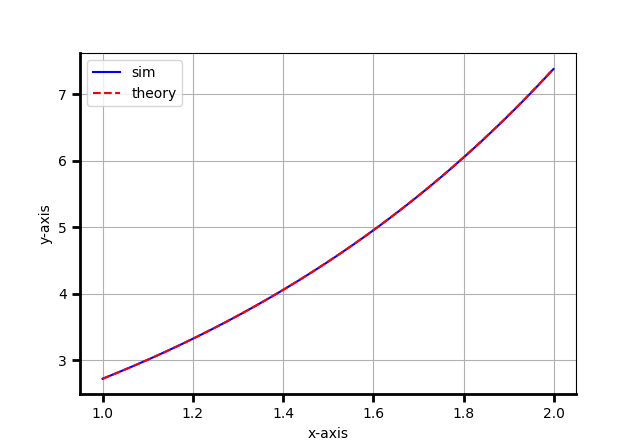
\includegraphics[width=\columnwidth]{fig/Figure_1.png}  
    \caption{Verification}
    \label{fig:example}  % Label for referencing
\end{figure}


\end{enumerate}

\end{document}

